%-----Main FIle------
%For Detail check out - http://firesofmay.blogspot.com/2011/10/latex-project-report-template
%CHANGE THESE Settings ONLY IF YOU KNOW WHAT YOU DOING

\documentclass[12pt,a4paper]{report}

%adjust your page margins here
\usepackage[top=0.70in, bottom=0.70in, left=0.8in,right=0.80in]{geometry} % setting the page alignment with this package
\usepackage[pdftex]{graphicx} %for embedding images
%\usepackage[hyphens]{url} %for proper url entries
\usepackage[dvips, bookmarks, colorlinks=false]{hyperref} %for creating links in the pdf version and other additional pdf attributes, no effect on the printed document
\usepackage[final]{pdfpages} %for embedding another pdf, remove if not required
\usepackage{float} %used for figure placement with H as a parameter
%\usepackage[hyphens]{url}
%\usepackage{hyperref}
\usepackage{pslatex} % for times new roman, old package, but works
\usepackage{array} % for making text bold in table


%For inserting Python Code
\usepackage{listings}
\usepackage{color}
 
\definecolor{dkgreen}{rgb}{0,0.6,0}
\definecolor{gray}{rgb}{0.5,0.5,0.5}
\definecolor{mauve}{rgb}{0.58,0,0.82}
 
\lstset{ %
  language=Python,                % the language of the code
  basicstyle=\footnotesize,           % the size of the fonts that are used for the code
  numbers=left,                   % where to put the line-numbers
  numberstyle=\tiny\color{gray},  % the style that is used for the line-numbers
  stepnumber=1,                   % each line is numbered
  numbersep=5pt,                  % how far the line-numbers are from the code
  backgroundcolor=\color{white},      % choose the background color. You must add \usepackage{color}
  showspaces=false,               % show spaces adding particular underscores
  showstringspaces=false,         % underline spaces within strings
  showtabs=false,                 % show tabs within strings adding particular underscores
  frame=single,                   % adds a frame around the code
  rulecolor=\color{black},        % if not set, the frame-color may be changed on line-breaks within not-black text (e.g. commens (green here))
  tabsize=2,                      % sets default tabsize to 2 spaces
  captionpos=b,                   % sets the caption-position to bottom
  breaklines=true,                % sets automatic line breaking
  breakatwhitespace=false,        % sets if automatic breaks should only happen at whitespace
  title=\lstname,                   % show the filename of files included with \lstinputlisting;
                                  % also try caption instead of title
  keywordstyle=\color{blue},          % keyword style
  commentstyle=\color{dkgreen},       % comment style
  stringstyle=\color{mauve},         % string literal style
  escapeinside={\%*}{*)},            % if you want to add a comment within your code
  morekeywords={*,...}               % if you want to add more keywords to the set
}

%%%%For inserting Python Code Over



%For the header and footer
\usepackage{fancyhdr}
\fancypagestyle{plain}{%
%\fancyhf{} % clear all header and footer fields
\fancyfoot[L]{\emph{This project is a Proof of Concept of Social Engineering Attack on Facebook using Web Scraping and Two Man in the middle attack Technique.}} % except the center
\fancyfoot[R]{\thepage}
\renewcommand{\headrulewidth}{0.4pt}
\renewcommand{\footrulewidth}{0.4pt}
}

\pagestyle{fancy}
\lhead{Chapter \thechapter}
\renewcommand{\chaptermark}[1]{% 
\markboth{#1}{}} 

\fancyfoot[LO,LE]{\emph{This project is a Proof of Concept of Social Engineering Attack on Facebook using Web Scraping and Two Man in the middle attack Technique.}}
\cfoot{}
\fancyfoot[RO, RE]{\thepage}
\renewcommand{\headrulewidth}{0.4pt}
\renewcommand{\footrulewidth}{0.4pt}
%For the header and footer Over

% Altering the Index Page Title
%\renewcommand{\contentsname}{\begin{center}\textsc{University Of Pune \\2011 - 2012}\\[1cm]Index\end{center}} 


%GLOBAL SETTINGS OVER, DOCUMENT BEGINS
\begin{document}

%Renames "Bibliography" to "References" on ref page
\renewcommand\bibname{References} 

%FROM HERE YOUR PAGES START GETTING ADDED

% includes the cover page
%2nd page after the title page

\newpage


\begin{center}
\thispagestyle{empty}


\Large{\textbf{A\\Project Report On}}\\[0.7cm]
\Large{\textsc {\textbf{SOCIAL ENGINEERING ATTACK BY PROFILE HIJACKING
AND USING HUMANS AS BOTNETS}}}\\[0.5cm]
%Example
%\Huge{\textsc {\textbf{A case study on linux}}}\\[1.0cm] % NOTE YOU HAVE TO REMOVE THE << >> ALSO!! That's just a placeholder here.
\Large{\textbf{Submitted By}}\\[0.5cm]
\begin{table}[h]
\centering
\begin{tabular}{>{\bfseries}lc>{\bfseries}r}
Mayank Jain & & B8058578\\ %Example B-1231414
Rahul Patil & & B8058598\\ %Example B-1231414
Anjali Shira & & B8058622\\ %Example B-1231414
\end{tabular}
\end{table}
\large{Under the guidance of}\\[0.5cm]
\Large{\textbf{Prof. S.C. Dharmadhikari}}\\[0.4cm]
\large{\emph{In partial fulfilment of}}\\
\LARGE{\textbf{Bachelor of Engineering}}\\
\LARGE{{[}B. E. Information Engineering{]}}\\[0.5cm]
\LARGE{{[}May 2012{]}}\\
\Large{\emph{AT}}\\[0.2cm]


% Bottom of the page

%MODIFY THE LOGO/DEPARTMENT NAME/COLLEGE NAME/ADDRESS IF YOU HAVE TO, ELSE LEAVE IT

\includegraphics[scale=0.5]{project/diagrams/pict_logo}\\
\large{\textbf{Department of Information Technology}}\\
\LARGE{\textbf{Pune Institute of Computer Technology}}\\
\Large{\textbf{Dhankawadi, Pune – 411043}}\\[0.5cm]
\Large{\textbf{Affiliated to}}\\[0.5cm]

\includegraphics[scale=5.0]{project/diagrams/uop-logo}\\
\LARGE{\textbf{University of Pune}}
\newpage

\end{center}

% Bottom of the page
%\begin{flushright}
%Faculty In-charge\\[1.5cm]
%Course Co-ordinator\\[1.0cm]
%\end{flushright}

%\begin{flushleft}
%Date:
%\end{flushleft}
 
\newpage

% includes the certificate page
%\chapter*{}
\begin{center}
\thispagestyle{empty}

\LARGE{\textbf{Pune Institute of Computer Technology}} \\ 
\large{\textbf{Department of Information Technology}}\\
\large{\textbf{Dhankawadi, Pune – 411043}}\\[0.5cm]


\includegraphics[scale=0.5]{project/diagrams/pict_logo}\\[0.5cm]

{\Huge \textbf{\emph{CERTIFICATE}}}\\[0.5cm]
\end{center}
\linespread{1.13}
\large{This is certify that the Dissertation entitled 
\textbf{``Social Engineering Attack By Profile Hijacking and Using Humans as botnets'',} 
submitted by 
\textbf{Mr. Mayank Jain}
 is a record of bonafide work carried out by him, in the partial
 fulfilment of the requirement for the award of Degree of Bachelor of
 Engineering (Information Technology) at Pune Institute of Computer
 Technology, Pune under the University of Pune. This work is done
 during year 2011-2012, under our guidance.}\\[1.0cm]
\large{---------------------------------}\\
\large{(Prof. S.C. Dharmadhikari)}\\[0.3cm]
\textbf{Project Guide}\\[1.0cm]
\large{--------------------------------}\hspace*{1.5in}\large{----------------------------------}\\
\large{Prof. Emmanual M.}\hspace*{2.0in}\large{Dr. P. T. Kulkarni}\\[0.3cm]
\textbf{HOD, IT Department}\hspace*{1.73in}\textbf{Principal PICT}\\[0.5cm]
\Large{\textbf{Examination:}}\\[0.8cm]
\large{Examiner ------------------------}\\[0.8cm]
\Large{\textbf{Date:}}
\newpage
 
\newpage

% includes the acknowledgements page
%\chapter*{}
\begin{center}
\thispagestyle{empty}
\LARGE{\textbf{Acknowledgements}}\\[1cm]
\end{center}
\linespread{1.13}
\large{I am profoundly grateful to \textbf{Prof. S.C. Dharmadhikari} for his expert guidance
and continuous encouragement throughout to see that this project rights its
target since its commencement to its completion.}\\[1cm]
\large{I would like to express deepest appreciation towards \textbf{Dr. P. T. Kulkarni},
Principal PICT, Pune, \textbf{Prof. Emmanual M.} HOD Information Technology
Department and \textbf{Prof. Manish R. Khodaskar} (Project Coordinator) whose
invaluable guidance supported me in completing this project.}\\[1cm]
\large{I am particularly grateful to \textbf{Dr. Navin Kabra}
(Punetech) who allows me to work in the company.\\[1cm]
\large{At last I must express my sincere heartfelt gratitude to all the staff members
of Information Technology Department who helped me directly or
indirectly during this course of work.}\\[3cm]
\large{\hspace*{4.5in} Mayank Jain}\\[0.25cm]
\large{\hspace*{4.5in} Rahul Patil}\\[0.25cm]
\large{\hspace*{4.5in} Anjali Shira}\\[0.25cm]
\newpage
 
\newpage

% includes the company 	certificate page
%\chapter*{}
\begin{center}
\thispagestyle{empty}
\vspace*{4\baselineskip}
\LARGE{\textbf{CERTIFICATE}}\\[1.0cm]
\large{This is to certify that the project report entitled}\\[0.7cm]
\Large{\textbf{Social Engineering Attack By Profile Hijacking and Using Humans as botnets}}\\[0.7cm]
\normalsize{Submitted by}\\[0.3cm]
\end{center}
\begin{table}[h]\large
\centering
\begin{tabular}{>{\bfseries}lc>{\bfseries}r}
Mayank Jain & & B8058578\\ %Example B-1231414
Rahul Patil & & B8058598\\ %Example B-1231414
Anjali Shira & & B8058622\\ %Example B-1231414
\end{tabular}
\end{table}
\normalsize{is a bonafide work carried out by them with the Sponsorship from ------------------- under the
\\supervision of Mr. ................................ and has been completed successfully .}\\[1.5cm]
\normalsize{(Mr. .................. )}\\
\normalsize{(Designation)}\\
\normalsize{External Guide}\\[1cm]
\normalsize{Place : Pune}\\
\normalsize{Date:}\\
\newpage
 
\newpage

\begin{center}
\thispagestyle{empty}
\vspace*{4\baselineskip}
\LARGE{\textbf{ABSTRACT}}\\[1.0cm]
\end{center}
\thispagestyle{empty}
\large{\emph{Social Engineering attack is a major security threat that needs to be
dealt. The only way to counter attack is to raise awareness among the users
of what all is possible in Social engineering attack and how it can be done.
We want to build a tool that will use Social Networking sites like facebook as
a platform to harnest the users data available and use that to impersonate
them via profile hijacking. Then we intend to use man in the middle attack
and make them reveal some information which is not available as a public
data. To test this we will use a modified version of the turing test.\\[1cm]}}
Keywords : Security, Social Networks, Facebook, Man in the middle attack % adds the Research Methodology page
\newpage

%TABLE OF CONTENTS AND LIST OF FIGURES ARE AUTOMATICALLY ADDED BY FOLLOWING COMMANDS
%ADD FIGURE OF TABLES IF YOU NEED TO, CHECK DOCUMENTATION
\pagenumbering{roman} %numbering before main content starts


%To reset the Header & Footer for TOC and LOF
\pagestyle{empty}
\addtocontents{toc}{\protect\thispagestyle{empty}}
\tableofcontents % adds Index Page

%\pagestyle{empty}

\addtocontents{lof}{\protect\thispagestyle{empty}}
\listoffigures % adds List of Figures
\cleardoublepage

%And reset back the settings we choose for Header and Footer
\pagestyle{fancy}

\newpage
\pagenumbering{arabic} %reset numbering to normal for the main content


%EACH CHAPTER CAN HAVE SECTIONS. EACH SECTION CAN HAVE MORE THAN ONE SUBSECTION AND EACH CHAPTER CAN HAVE MORE THAN ONE SECTION
%EXAMPLE
% \chapter{Introduction}
% \section{Need}
% \subsection{Social Engineering}


\chapter{Introduction}

\section{Need}

\subsection{Social Engineering}
Social Engineering is the act of manipulating a person to take an action that
may or may not be in the targets best interest. This may include obtaining
information, gaining access, or getting the target to take certain action\cite{book_se}

\subsection{Current Scneario}
Businesses spend a significant portion of their annual information technology
budgets on high-tech computer security. But the firewalls, vaults, bunkers,
locks and biometrics those dollars buy can be pierced by attackers targeting
untrained, uninformed or unmonitored users. Humans are the weakest link in
any security system, according to KL-based organizers of the Hackers Halted
Asia Pacific 2009 conference.\cite{link_humanweak}\\[0.5cm]
The chief minister of Malacca, Datuk Seri Haji Mohd Ali Bin Mohd Rus-
tam, said there is no perfect system in the world. ”Even if you have the best
security devices and software–your organization still relies on humans–who
are the weakest link in any security system. Public education and awareness
is essential.”\\[0.5cm]
Figure \ref{fig:data} is a Data Security Breach Statistics of 2008 revealing that
Malicious Insider and Careless/Untrained Insider is a bigger threat than an
outside cracker.\\[0.5cm]
Also, in the age of Social Networking Sites like Facebook, Twitter, Linkedin,
Google+ information of companies internal hierarchy structure, employees,

\begin{figure}[htb]

\centering
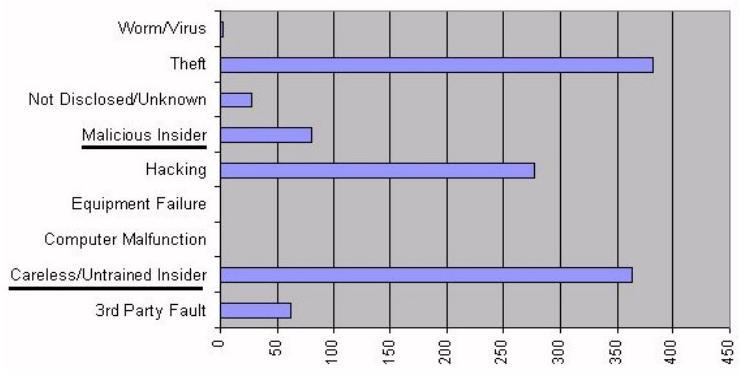
\includegraphics[scale=0.6]{project/figdata}
\caption{Figure 1.1: Data Security Breach Statistics of 2008}
\label{fig:data} %see below of how to use it
\end{figure}

personal information is readily available online for the information gathering
phase to breach companies security perimeter by various social engineering
ways like phishing links, Trojans, Backdoors, Password guessing, breaking
security questions etc.\\[0.5cm]
Is it possible to break into the circle of friends network on social networking
sites and make them reveal certain information about them which can be
used further to infiltrate the security perimeter of a company?\\[0.5cm]
Our project is designed to answer this Question and provide a Proof of Con-
cept that Yes, it can be done and without even raising any suspicion on the
target for a long time.


%\ref is used to refer to the \label of an image, below is an example
%Figure \ref{fig:data} is a Data Security Breach Statistics of 2008 revealing that Malicious Insider and Careless/Untrained Insider is a bigger threat than an outside cracker.
%BLAH BLAH

\section{Basic Concept}
In this project we will use two main concepts:

%BLAH BLAH
\subsection{Profile Hijacking}
%BLAH BLAH

In Profile Hijacking, we will impersonate the target(s) profile on Social Net-
working Sites like Facebook and use their identity to infiltrate the network
of other targets friend to fit in the group. Profile Hijacking is important, to
use them to reveal certain information without their knowledge.\cite{paper_allyourcontacts}


\subsection{Using Humans as Botnets}
%BLAH BLAH

We studied many AI based Chat Bots that are available on the web and
we found that Using Chat Bots to chat with humans for Social Engineering Attack is not feasible as Humans detect that the other person is not a
human but a program and hence the attack fails even before it is launched.\cite{paper_towardsautomating}\\[0.5cm]
Since developing a fully convincing AI based Chat Bot is not possible consid-
ering the Scope, we will use another human to do the talking with our target
while we sit in between, watch and modify the conversation towards the
conversation which would reveal certain information which we are interested
in.\cite{paper_honeybot}


\section{Application}
%BLAH BLAH
Some of the best tools for fighting social engineering attacks are security
awareness training and social engineering testing. The effectiveness of these
controls will vary based on the quality of their implementation, including
follow-up and retraining.\\[0.5cm]
Social engineering testing, by its very nature, can be difficult to conduct
without third-party assistance. One option is to engage an information secu-
rity organization to conduct testing. The testing can uncover areas in which
an organization is most vulnerable so that risk can be assessed and mitiga-
tion strategies can be formulated and implemented.\\[0.5cm]
Rolling social engineering testing into a larger security penetration engage-
ment can reduce the cost of the social engineering component, says Jim
Patterson, director of consulting for Rapid7.\cite{link_humanweak}\\[0.5cm]
Main Application of this Project is to develop a tool that will aid in Do-
ing Social Engineering Testing on Companies Employees, also it will provide
as a live demonstration to employees under training on how social engineer-
ing can be done and how by being cautious one can prevent serious damage
not only to the company but also to their private life.\\[0.5cm]
 % adds the introduction page
\chapter{Literature Survey}

%First paper
%Example :
%\section[Towards AES using SNS]{Towards Automating Social Engineering Using Social Networking Sites}
%Note short names are optional, for it to show shorter name in table of contents if its too long.
\section{Towards Automating Social Engineering Using Social Networking Sites}

\subsection{Summary}

In this paper, we saw the use of artificial intelligence to create a chat bot
to do the automatic social engineering attack via social networking sites.
Experiments were done on a small group of people on facebook.


\subsection{Advantages}

%This is how you write things in bullet points
\begin{itemize}
\item{Automatic tool, minimal input required from the user.}
\item{If perfected, could be the best way to automate social engineering attack.}

\end{itemize}

\subsection{Disadvantages}

%This is how you write things in bullet points
\begin{itemize}
\item{Fails to convince that the chat bot is a real human.}
\item{Has no input of real world information.}
\item{Chat algorithm is hard coded using regular expressions.}
\item{No real world testing because of ethical issues.}
\item{Building a real world chat bot is out of scope.}

\end{itemize}

%Add Second paper

\section{All Your Contacts Are Belong to Us: Automated Identity Theft Attacks on Social Networks}
\subsection{Summary}

Presents a novel concept of profile hijacking and cloning, which laid the
foundation for the proposed idea.

\subsection{Advantages}
%This is how you write things in bullet points
\begin{itemize}
\item{Works with all social networking sites which has no authentication mechanism of who you say is who you are in real world.}
\item{Very Easy to do, as most of the data required is already available.}

\end{itemize}

\subsection{Disadvantages}
%This is how you write things in bullet points
\begin{itemize}
\item{Does not give us information which is not available directly.}
\item{Impersonating or Faking a human identity is a punishable act.}
\item{Real world testing has ethical issues.}

\end{itemize}


%Add Third Paper
\section{Honeybot, Your Man in the Middle for Automated Social Engineering}
\subsection{Summary}

This paper presents the basic idea we can do man in the middle attack on two
users. The testing was done on public IRC’s but was suggested that it can
be done by using profile hijacking on a social networking sites like Facebook.

\subsection{Advantages}
%This is how you write things in bullet points
\begin{itemize}
\item{Results of success is much higher than by using artificial intelligence via a chat bot.}
\item{Easy to build compared to building artificial intelligence.}

\end{itemize}

\subsection{Disadvantages}
%This is how you write things in bullet points
\begin{itemize}
\item{Required gender conversion in IRC’s chat when impersonating a different gender.}
\item{Testing was done on IRC’s which is not targetted information gathering.}

\end{itemize}

%Add Fourth Paper


\section{Eight Friends Are Enough Social Graph Approximation via Public Listings}
\subsection{Summary}

Presents a novel idea of Publically available data of users on social networking
sites. Also presents the idea of Dominating Sets. It was also mentioned that
the facebook friends public data policy keeps changing, before it was 10
friends than it became 8 and now again its back to 10.


\subsection{Advantages}
%This is how you write things in bullet points
\begin{itemize}
\item{Avoids detection by Facebook.}
\item{Presents a novel idea of using Dominating Sets.}

\end{itemize}

\subsection{Disadvantages}
%This is how you write things in bullet points
\begin{itemize}
\item{Is not succesful in the current scenario where users are security concious.}
\item{Has very low sucess rate as per our experiments.}

\end{itemize} % adds the Literature Survey page
\chapter{Proposed Work}

\section{Problem Statement}
\emph{To develop a tool which can be used for automated social engineering attack on users of social networking sites using profile hijacking and man in the middle attack. Also test the tool via modified version of Turing test at basic conversation level}

\section{Passive Information Gathering Module}

\subsection{Social Networks}
A social networking service is an online service, platform, or site that focuses on building and reflecting of 
social networks or social relations among people, who, for example, share interests and/or activities and people 
with similar or somewhat similar interests, backgrounds and/or activities make their own communities.\\[0.5cm]
A social network service consists of a representation of each user (often a
profile), his/her social links, and a variety of additional services.\\[0.5cm]
According to ComScore, Facebook has the largest number of Social Network User shares (up to end of November 2011)\cite{marketshare}

\begin{table}[h]\large
\centering
\begin{tabular}{l | c | r}
Worldwide & Unique Visitors & Percentage\\
Facebook.com & 792,999 	& 55.1\%\\
Twitter.com & 167,903 & 11.7\%\\
LinkedIn.com & 94,823 & 6.6\%\\
Google Plus & 66,756 & 4.6\%\\
MySpace & 61,037 & 4.2\%\\
Others & 255,539 & 17.8\%\\
Total & 1,438,877 & 100\%\\
\end{tabular}
\end{table}

And here are some statistics about Facebook (Alexa estimates, as of  20/04/2012) :-
\begin{itemize}
\item{daily page views : ~8.4 billion}
\item{daily visitors : ~650 million}
\item{views per visitor : 12.9}
\item{site rank : 2nd}
\item{traffic fraction : 0.45\% ~1  in  220   of all web traffic }
\end{itemize}


This shows that there is a lot of user generated information that is available to tap into. Facebook has its own API but we 
cannot use that to extract data about anyone. So we thought of writing a module which can do Web Scraping.
%Below is an example of how you will add references. short_paper_name is what you have specified in your ref.tex file
% so it will automatically do the [5] for you, or whatever number it is.

\subsection{Web Scraping}
Web scraping (also called web harvesting or web data extraction) is a computer software technique of extracting information from 
websites. Usually, such software programs simulate human exploration of the World Wide Web by either implementing low-level Hypertext 
Transfer Protocol (HTTP), or embedding a fully-fledged web browser, such as  Internet Explorer or Mozilla Firefox.\cite{wiki_scraping}

\subsection{Features}
This module will have the ability to scrape contents of facebook profile users page. It'll basically focus on the friends list of a user.
The data generated from this module will help in focusing on who are the victims friends, what are the statistics of them etc.\\[0.5cm]
Figure \ref{fig:myfriends} is a screenshot of a user and his friends list
\begin{figure}[htb]
\centering
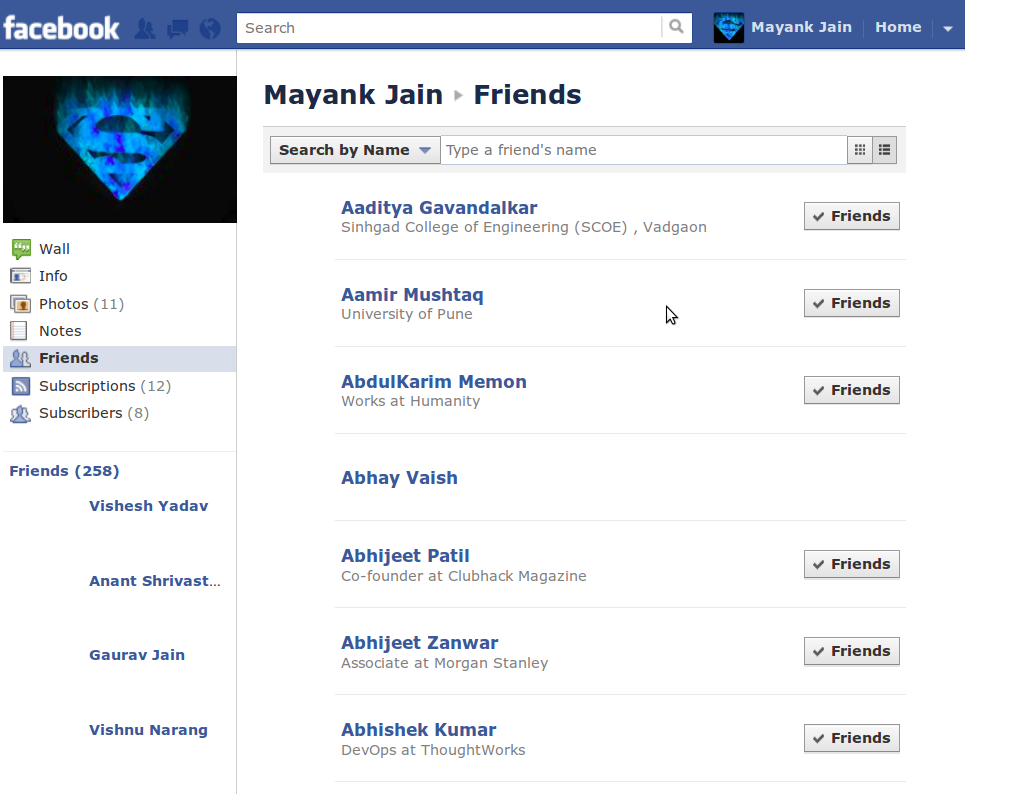
\includegraphics[scale=0.4]{project/diagrams/myfriends}
\caption{Friends List on Facebook}
\label{fig:myfriends} %see below of how to use it
\end{figure}

This module should be able to extract\\
\begin{itemize}
\item{Full Name}
\item{Gender : Male/Female/NA}
\item{username : Username/NA}
\item{Number of Friends : Total/NA}
\item{Unique UserID}
\end{itemize}

And in addition it should be able to extract each user's friends detail in a BFS Manner. And it can continue this as long as we want it to.

\section{Facebook Chat Attack Module}
\subsection{Extensible Messaging and Presence Protocol}
Extensible Messaging and Presence Protocol (XMPP) is an open-standard communications protocol for message-oriented middleware based on 
XML (Extensible Markup Language). The protocol was originally named Jabber, and was developed by the Jabber open-source community 
in 1999 for near-real-time, extensible instant messaging (IM), presence information, and contact list maintenance. Designed to 
be extensible, the protocol today also finds application in VoIP and file transfer signaling.\cite{wiki_xmpp}

Facebook uses XMPP (Extensible Messaging and Presence Protocol) for chatting.	


\subsection{Attack as Example}
  Following is an example.\\
Lets say we have two marks (targets) Alice (Human) - aliceHuman and Bob
(Human) - bobHuman\\[0.5cm]
We make two profiles both run by bots. The highlight is bothbots hijack the
profilesof marks namely alice and bob.\\[0.5cm]
So aliceBots profile is similar to aliceHumans profile and bobBot’s profile
is simlar to bobBot’s profile. aliceBotsends a friend request to bobHuman.
bobBotsends a friend request to aliceHuman. So now, aliceHuman is a friend
of bobBot and bobHuman is a friend of aliceBot. Also, bobBot and aliceBot
can exchange information outside of facebook to each other.\\[0.5cm]
So now lets say, bobHuman and aliceHuman are online. Our bots start
the conversation. Whatever is being passed to one of the Bot by one human,
it is passed on to the other Bot and in turn passed on to the other human,
i.e. two humans are having conversation through two bots but they think
that they are talking to a human since the conversation sounds like a human
(which it is).\\[0.5cm]
After some amount of bonding between them our bots start modification
by using injecting questions inside the conversations\\[0.5cm]\newpage
\noindent
\textbf{AliceHuman - bobBot} : ”Hey how was the movie yesterday?”\\
\textbf{botBot - aliceBot} : ”Hey how was the movie yesterday?and hey btw whats
your fav color?”\\
\textbf{aliceBot - BobHuman} : ”Hey how was the movie yesterday? and hey btw
whats your fav color?”\\[0.5cm]
\textbf{BobHuman - aliceBot} : ”movie was great, and its blue btw, whats yours?”\\
\textbf{aliceBot - bobBot} : ”movie was great,you know my fav color is blue, what is yours?”\\
\textbf{bobBot - AliceHuman} : ”movie was great, you know my fav color is blue, what is yours?”\\[0.5cm]
\textbf{AliceHuman - bobBot} : ”mine is pink :)”\\
\textbf{botBot - aliceBot} : ”mine is pink :)”\\
\textbf{aliceBot - BobHuman} : ”mine is pink :)”\\[0.5cm]

Notice how the conversation has been altered to make it unclear that no
one asked each other about favorite color and yet both of them told us their
favorite color. We got hold of two marks information without raising suspicion.\\[0.5cm]


\begin{figure}[htb]
\centering
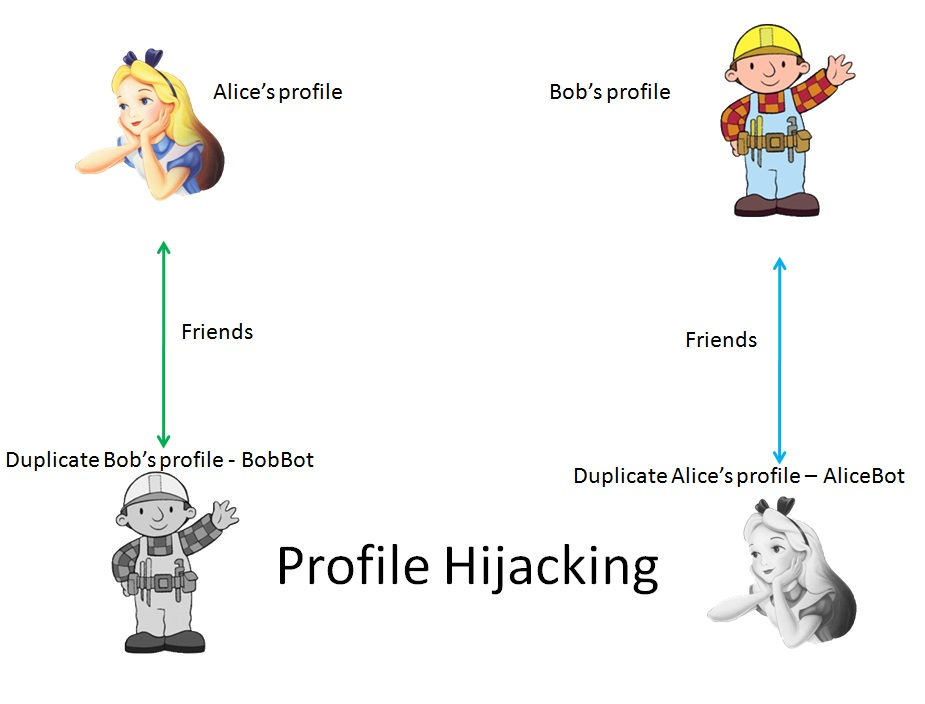
\includegraphics[scale=0.4]{project/diagrams/chatattack1}
\caption{Example of Profile Hijacking}
\label{fig:chatattack1} %see below of how to use it
\end{figure}

\begin{figure}[htb]
\centering
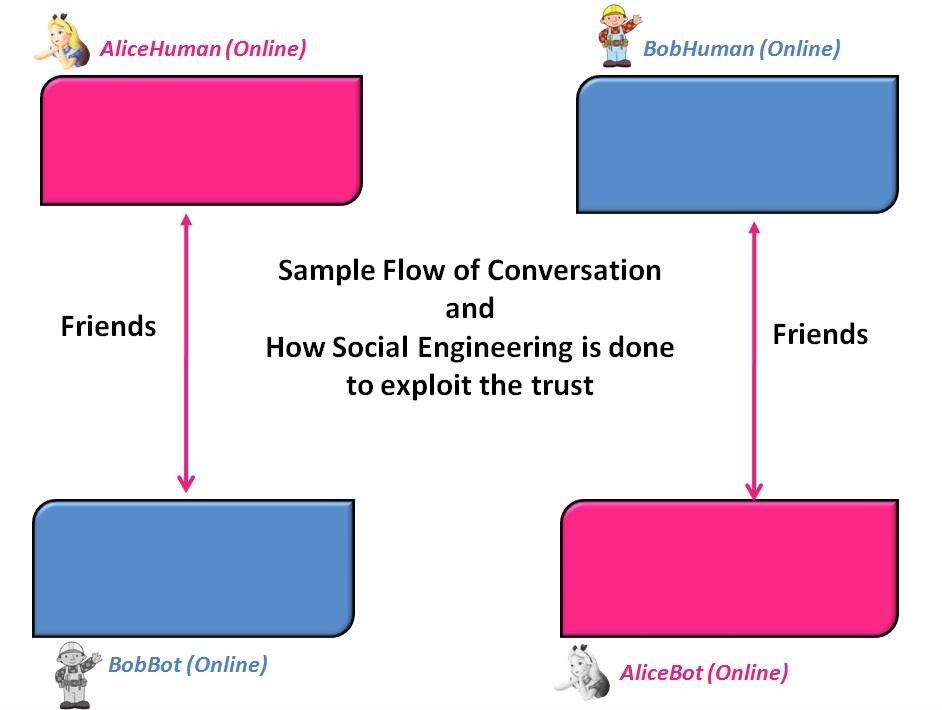
\includegraphics[scale=0.4]{project/diagrams/chatattack2}
\caption{Example of Conversation Modification - 1}
\label{fig:chatattack1} %see below of how to use it
\end{figure}

\begin{figure}[htb]
\centering
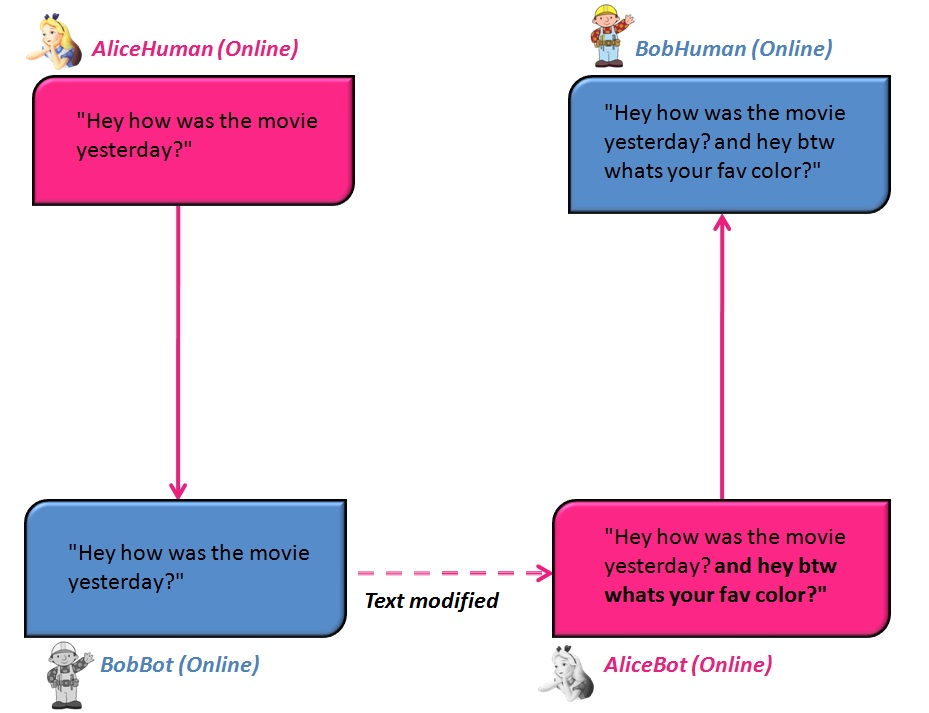
\includegraphics[scale=0.4]{project/diagrams/chatattack3}
\caption{Example of Conversation Modification - 2}
\label{fig:chatattack3} %see below of how to use it
\end{figure}

\begin{figure}[htb]
\centering
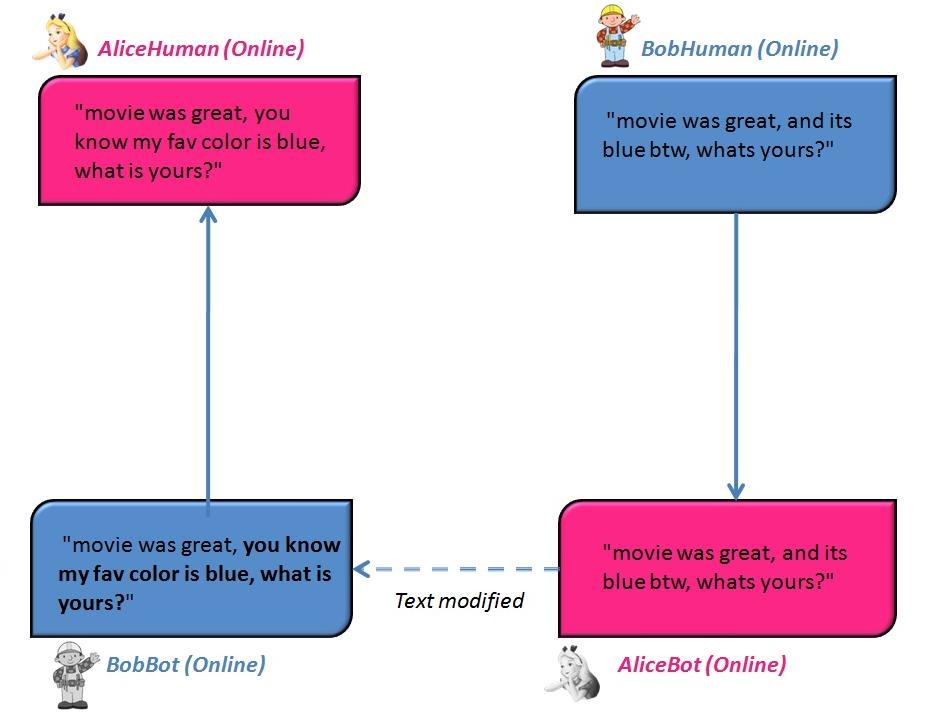
\includegraphics[scale=0.4]{project/diagrams/chatattack4}
\caption{Example of Conversation Modification - 3}
\label{fig:chatattack4} %see below of how to use it
\end{figure}

\begin{figure}[htb]
\centering
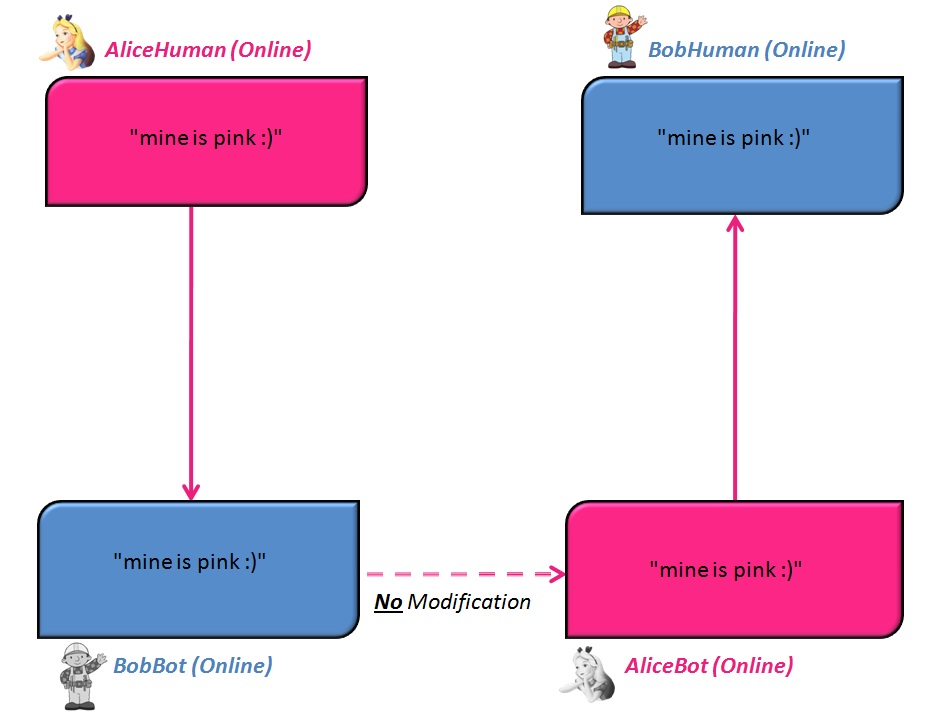
\includegraphics[scale=0.4]{project/diagrams/chatattack5}
\caption{Example of Conversation Modification - 4}
\label{fig:chatattack5} %see below of how to use it
\end{figure}


\subsection{Constraints}
We will develop a POC (Proof of Concept) only. To modify the conversation we will use simple regex based parsing to match and substitute
it with matching strings. There will be no Artificial Inteligence or Machine Learning involved as that is out of scope at this level. Though 
it can be done and will make the modification more scalable and justified. % adds the Project Work page
\chapter{Research Methodology}

\section{Passive Information Gathering Module}

\subsection{HTTP}
To implement Web Scraping module for Information Gathering we need to understand the HTTP protocol. HTTP (The Hypertext Transfer 
Protocol) is an application protocol for distributed, collaborative, hypermedia information systems. HTTP is the 
foundation of data communication for the World Wide Web.

\subsubsection{Request methods}
HTTP defines nine methods (sometimes referred to as "verbs") indicating the desired action to be performed on the identified 
resource. What this resource represents, whether pre-existing data or data that is generated dynamically, depends on the 
implementation of the server. Often, the resource corresponds to a file or the output of an executable residing on the server.\\[0.5cm]
Following are the main request methods we will be dealing with :-
\begin{description}
\item[POST : ] Submits data to be processed (e.g., from an HTML form) to the identified resource. The data is included in the body of the request. This may result in the creation of a new resource or the updates of existing resources or both.
\item[GET : ] Requests a representation of the specified resource. Requests using GET should only retrieve data and should have no other 
effect. (This is also true of some other HTTP methods.) The W3C has published guidance principles on this distinction, saying, 
"Web application design should be informed by the above principles, but also by the relevant limitations."
\end{description}

\subsection{urllib2}
Since we will be using Python 2.x for our project, we will be using the standard library for doing the HTTP requests to be made.
The urllib2 module defines functions and classes which help in opening URLs (mostly HTTP) in a complex world — basic and digest authentication, redirections, cookies and more.\cite{py_urllib2}

urllib2.urlopen(url[, data][, timeout])\\[0.5cm]

\emph{ - Open the URL url, which can be either a string or a Request object.}

\subsection{Regular Expressions}
A Regular Expression is the term used to describe a codified method of searching invented, or defined, by the American mathematician Stephen Kleene.\cite{whatisregex} % adds the Research Methodology page
\chapter{Project Design}


\section{Use Case diagrams}
\subsection{Use Case - System Component}

%add your use case diagrams here

\begin{figure}[H]
\centering
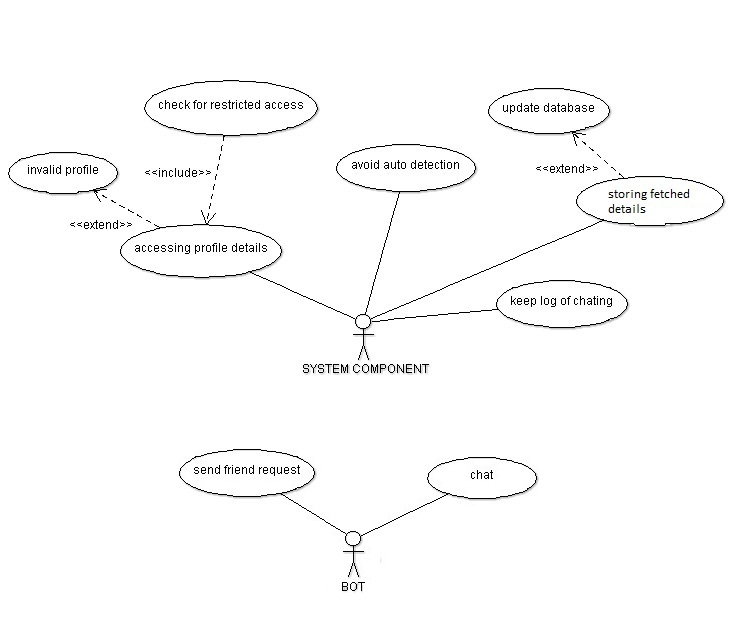
\includegraphics[scale=0.7]{project/diagrams/usecase1}
\caption{Use Case Diagram - System Component}
\label{fig:usecase1}
\end{figure}

\begin{figure}[H]
\centering
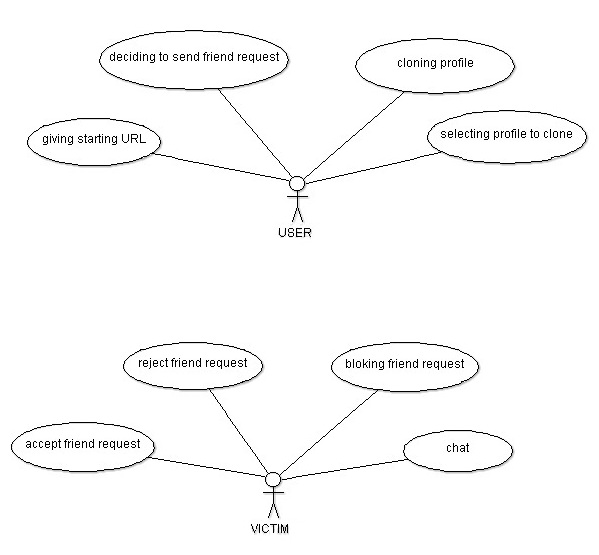
\includegraphics[scale=0.8]{project/diagrams/usecase2}
\caption{Use Case Diagram - Victim and User}
\label{fig:usecase2}
\end{figure}

\begin{figure}[H]
\centering
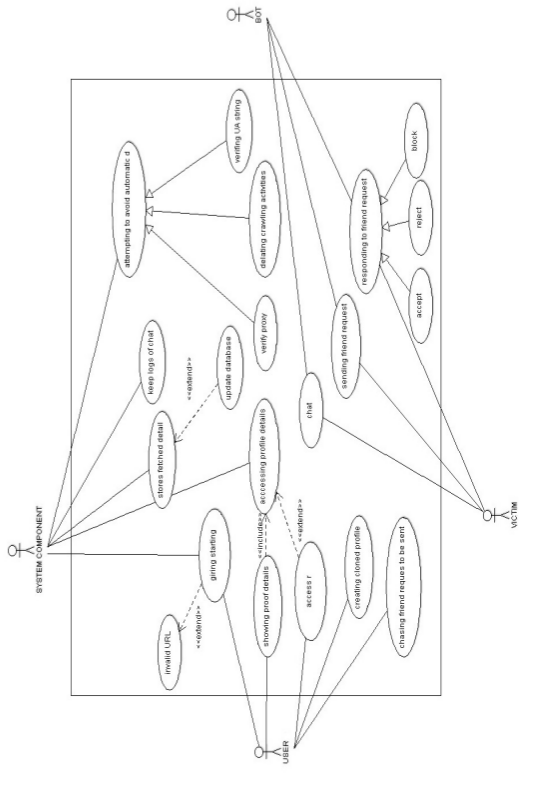
\includegraphics[scale=1.0]{project/diagrams/usecase3}
\caption{Use Case Diagram - Main}
\label{fig:usecase3}
\end{figure}


%Add more if you have to with copy pasting subsections


%add your ER diagrams here
\section{ER Diagram}


\begin{figure}[H]
\centering
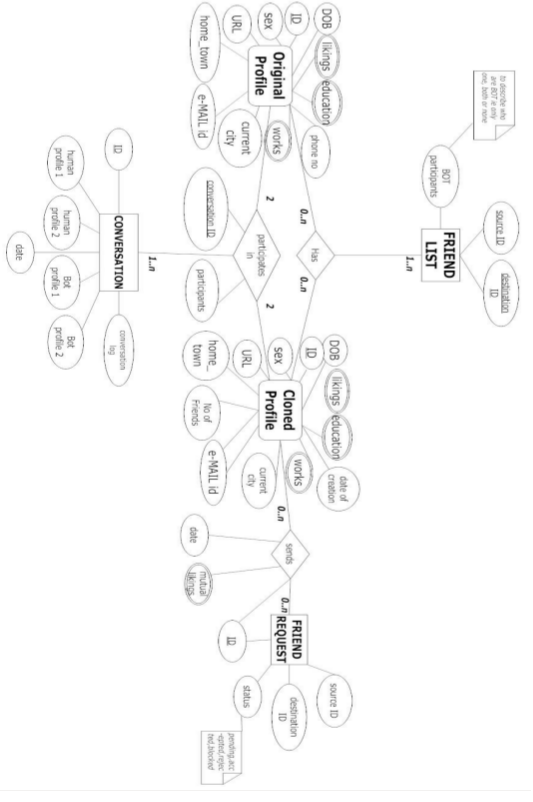
\includegraphics[scale=1.0, angle=180]{project/diagrams/er1}
\caption{ER Diagram}
\label{fig:er}
\end{figure}



\section{DFD (level 0/1/2)}

\subsection{DFD Level 0}

\begin{figure}[H]
\centering
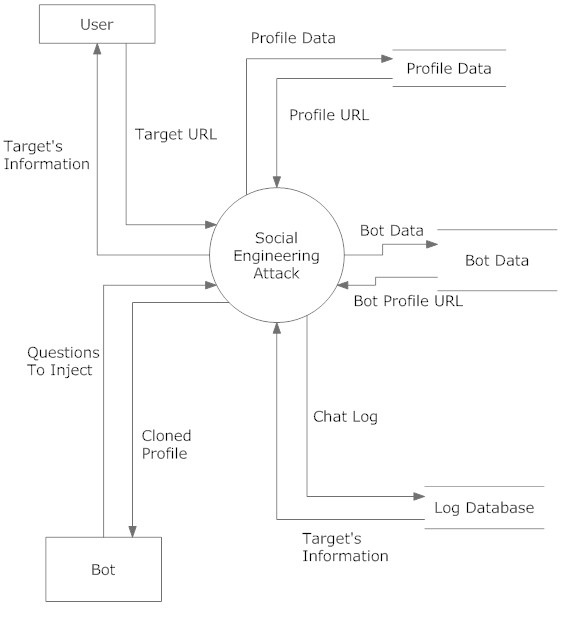
\includegraphics[scale=0.8]{project/diagrams/dfd0}
\caption{DFD - Level 0}
\label{fig:dfd0}
\end{figure}

\subsection{DFD Level 1}

\begin{figure}[H]
\centering
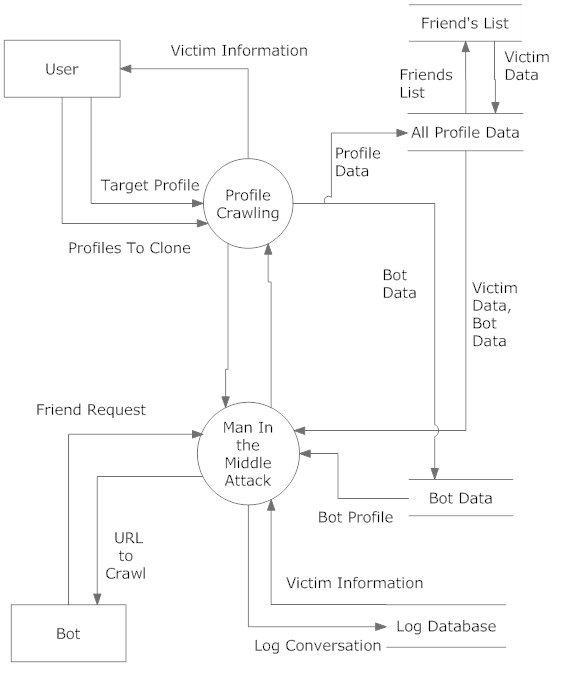
\includegraphics[scale=0.8]{project/diagrams/dfd1}
\caption{DFD - Level 1}
\label{fig:dfd1}
\end{figure}

\subsection{DFD Level 2}

\begin{figure}[H]
\centering
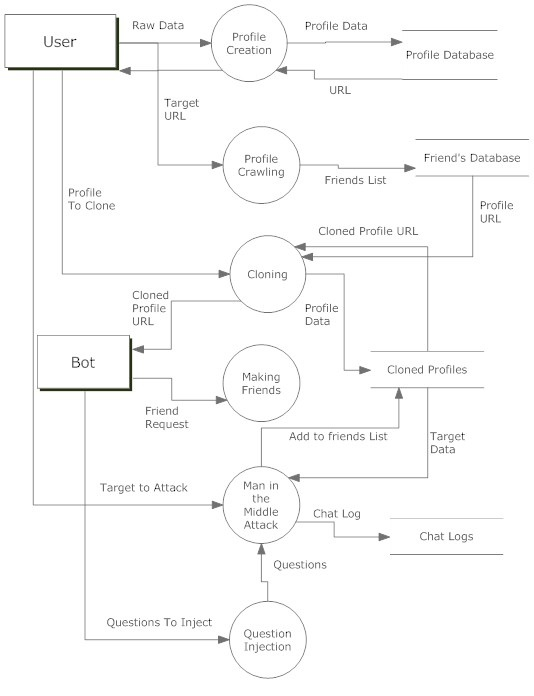
\includegraphics[scale=0.8]{project/diagrams/dfd2}
\caption{DFD - Level 2}
\label{fig:dfd2}
\end{figure}

\section{Activity Diagram}

\begin{figure}[H]
\centering
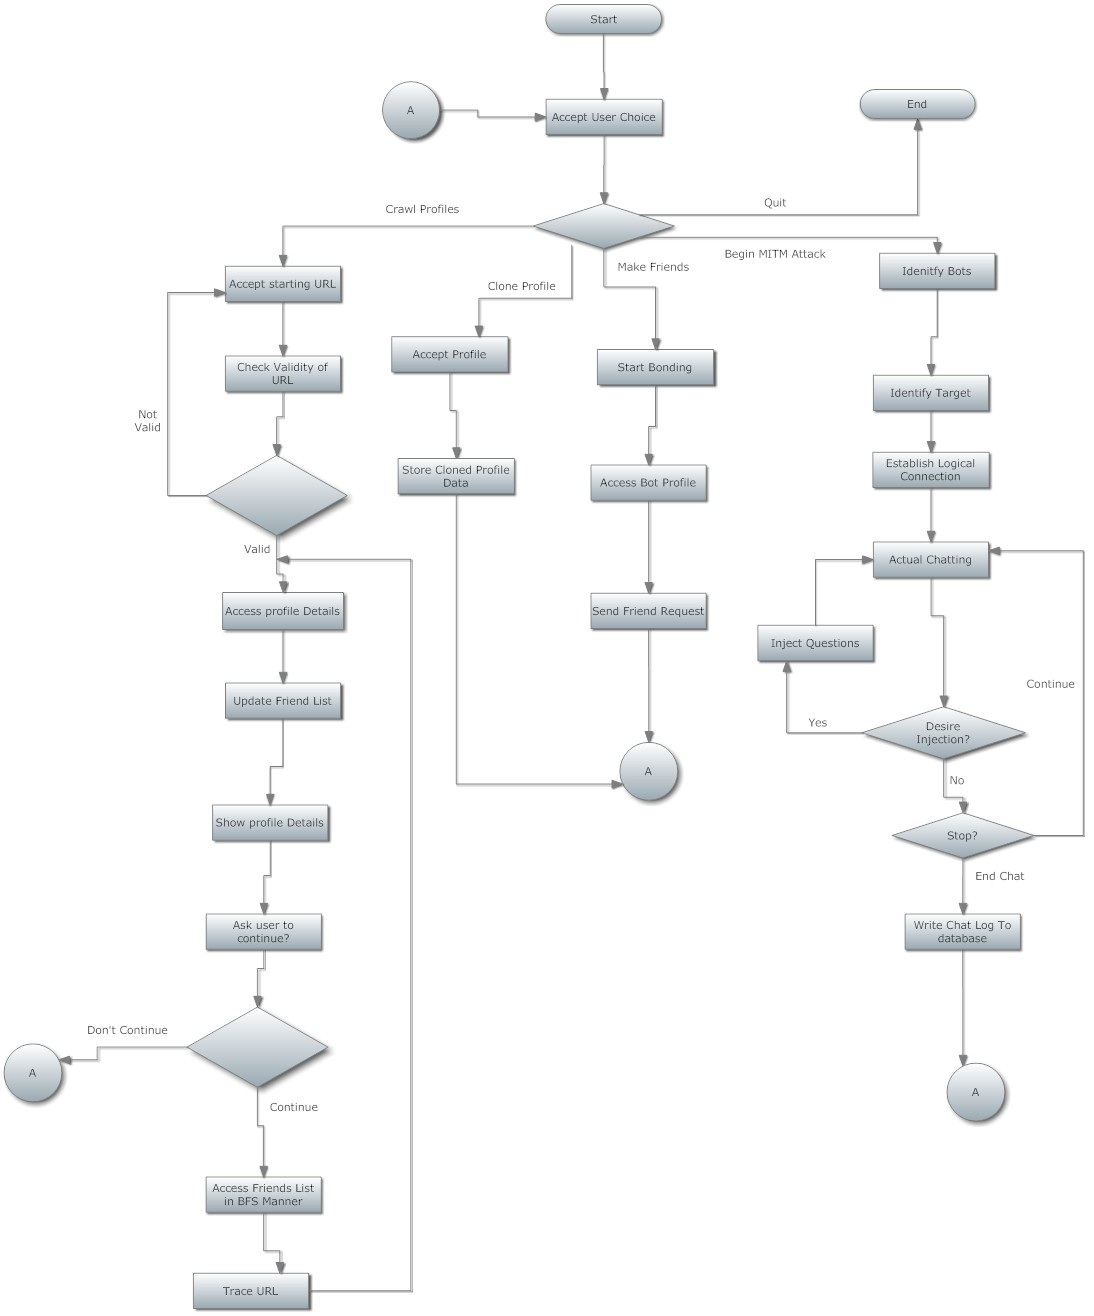
\includegraphics[scale=0.45]{project/diagrams/activity}
\caption{Activity Diagram}
\label{fig:activity}
\end{figure}


\section{Hardware and software requirements}
\subsection{Hardware}

%Add your items here
\begin{itemize}
\item{Standard Desktop Computer}
\item{2 GB Ram}
\item{80GB Hard Disk}
\item{Internet Connection}
\end{itemize}
\subsection{Software}

%This is how you add bullet points without a bullet
\begin{description}
\item[Operating System : ]  Any Linux based distro
\item[Language : ] Python 2.x
\item[Regular Expression : ] Python's re Library
\item[HTTP Requests : ] Python's urllib, urllib2 Library
\item[XMPP : ] Python's SleekXMPP Library
\end{description}

 % adds the Project Design
\chapter{Implementation}

\section{Passive Information Gathering Module}

\subsection{Database Connections}
Following snippet initializes the database connections :-
\lstinputlisting{project/code/initdbconfig.py}

This code creates the two Tables :-
\lstinputlisting{project/code/initializedb.py}

\subsection{Facebook Login}
To implement scraping, we needed to login via the script. Following is the snippet 
\lstinputlisting{project/code/LoginFB.py}

\subsection{Fetching Friends}

Following Code fetches Friends list of a user.
\lstinputlisting{project/code/FetchFriends.py}
And Following is a sample of data collected of a Facebook User.\\
\begin{table}[h]
\centering
\begin{tabular}{>{\bfseries}l>{\bfseries}c>{\bfseries}r}
Attributes	& 	User1 			& UserN\\
Seq Id		& 	1 			& 3\\
Profile ID      & 	100002012773778 	& 698854997\\
Full Name	& 	Hemant Rathore		& Ashish Chauhan\\
Usrname 	& 	NA			& chauhan.ashish\\
Frnds           &	35			& 1356\\
TimeStamp 	&	2011-12-26 01:42:02	& 2011-12-26 03:28:44\\
Scrapped 	&	35			& 1280\\
IsDone 		& 	1 			& -1\\
Level    	& 	0  			& 1\\
Sex		& 	male 			& male\\
\end{tabular}
\end{table}

\newpage

\subsection{Summary of Data}

\begin{description}
\item[Target Profile ID :]  100002012773778
\item[Username :] NA
\item[Name :] Hemant Rathore
\item[Gender :] Male
\item[Profile Link :] http://www.facebook.com/profile.php?id=100002012773778\\
\item[Total Friends of Hemant Rathore                       (Level 1):]  35
\item[Total Friends of Friends of Hemant Rathore            (Level 2):]  7443
\item[Total Friends of Friends of Friends of Hemant Rathore (Level 3):]  17,73,288\\
\item[Number of Males   at Level 1:] 30
\item[Number of Females at Level 1:] 3
\item[Number of NA      at Level 1:] 1 \\
\item[Number of Males   at Level 2:] 4420
\item[Number of Females at Level 2:] 1241
\item[Number of NA      at Level 2:] 97\\
\item[Number of People who have hidden their Friends list at Level 1:] 11/35
\item[Number of People who have hidden their Friends list at Level 2:] 1733/7443\\
\item[Total Number of People who have hidden their Friends list:] 1744/7478 Approx 25\% Only.
\item[Total Number of People who Do NOT have usernames set:] 3128/7478 = 40\% Approx
\item[Total Number of People who Have Hidden their Gender:] 98/7478 = 1\% Approx\\
\item[Run Duration:] 473 Mins.
\item[Friends Fetched/Min:] (7443+35) / 473 = 15 Frnds/mins (rounded off)\\
\item[Data Base Size:] 0.94989872 MB\\
\item[Number of Unique friends edges found:] 6613
\item[Number of Unique Profiles found:] 5793
\end{description}
                                                                    
\section{Facebook Chat Attack}

Following is a snippet of Chat Replay and Modification Code
\lstinputlisting{project/code/alexbot.py}

and following are the screenshots of the attack

\begin{figure}[H]
\centering
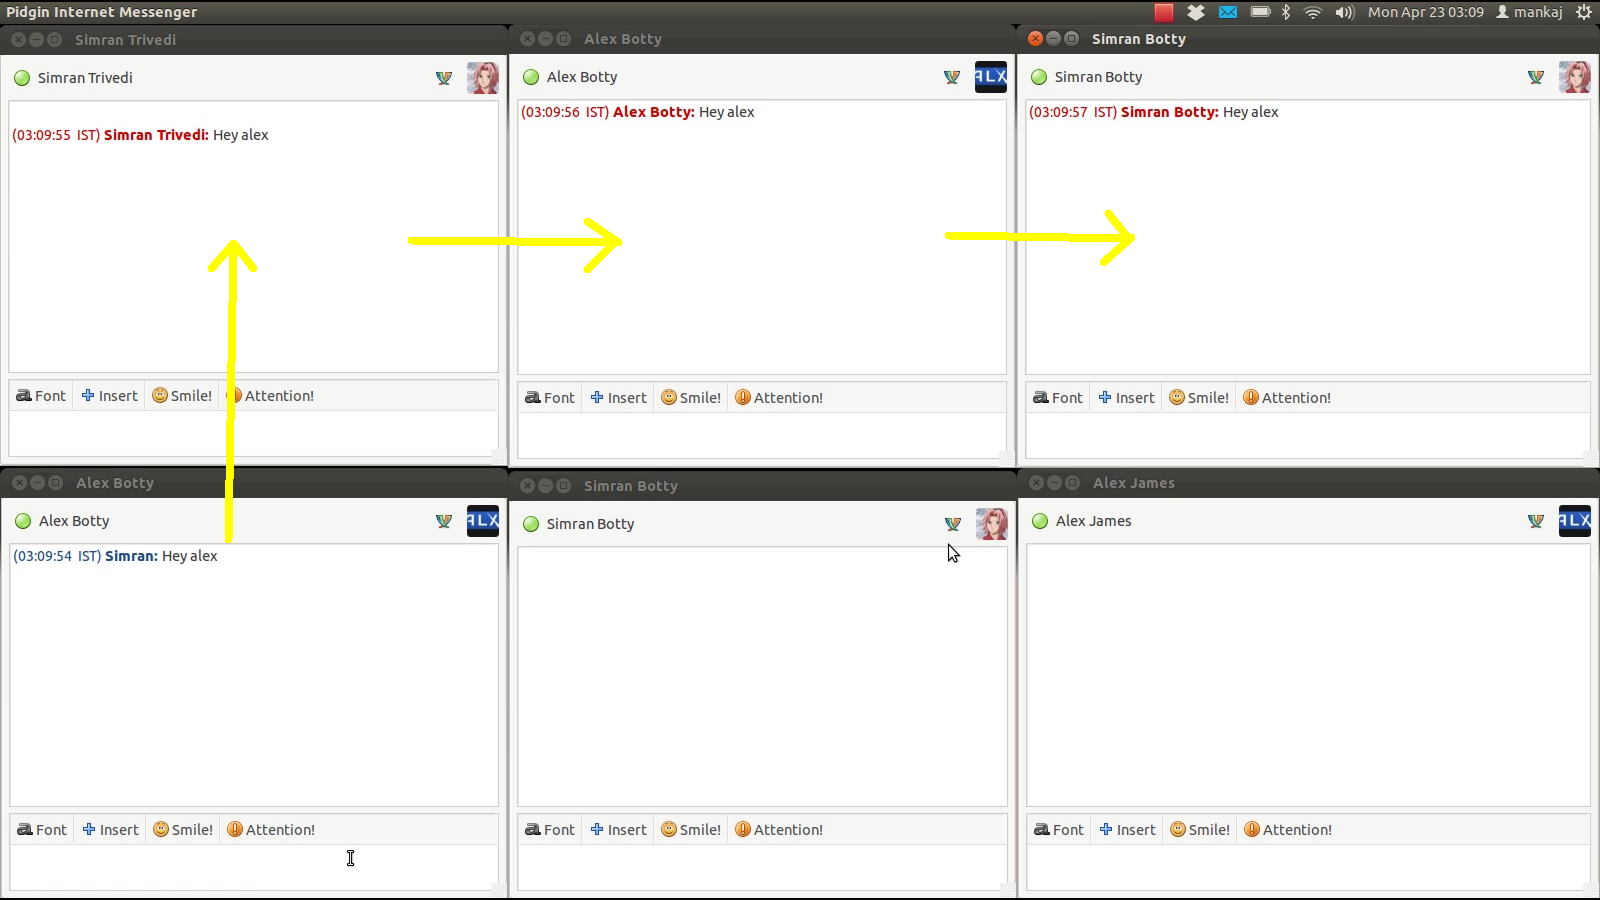
\includegraphics[scale=0.6, angle=90]{project/diagrams/attack1}
\caption{Facebook Chat Attack - 1}
\label{fig:attack1}
\end{figure}

\begin{figure}[H]
\centering
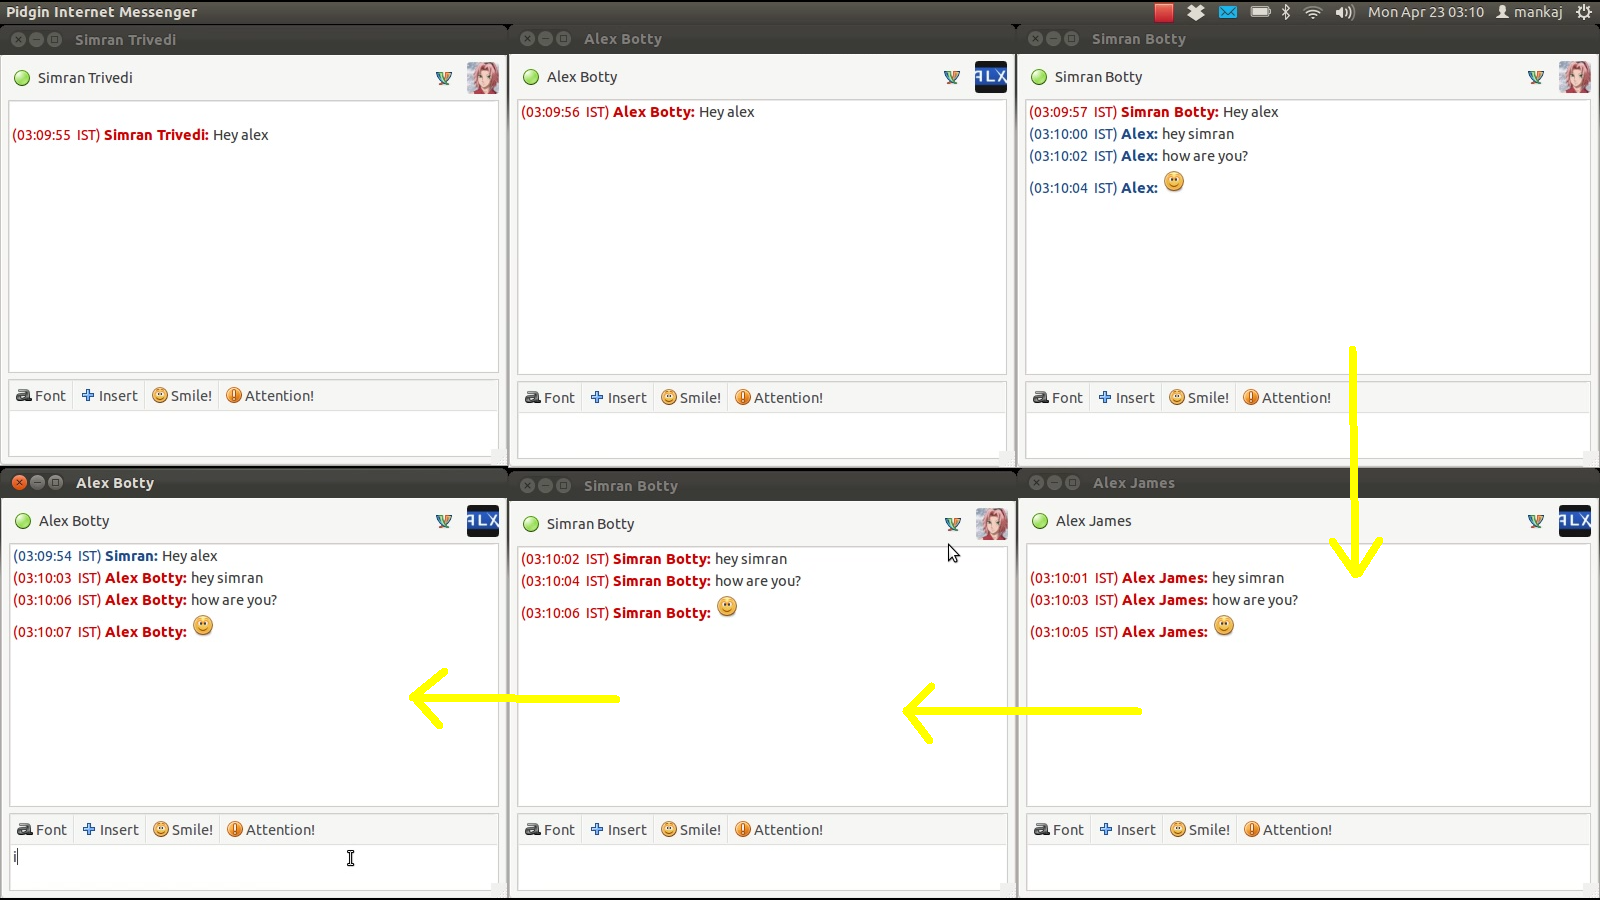
\includegraphics[scale=0.6, angle=90]{project/diagrams/attack2}
\caption{Facebook Chat Attack - 2}
\label{fig:attack1}
\end{figure}

\begin{figure}[H]
\centering
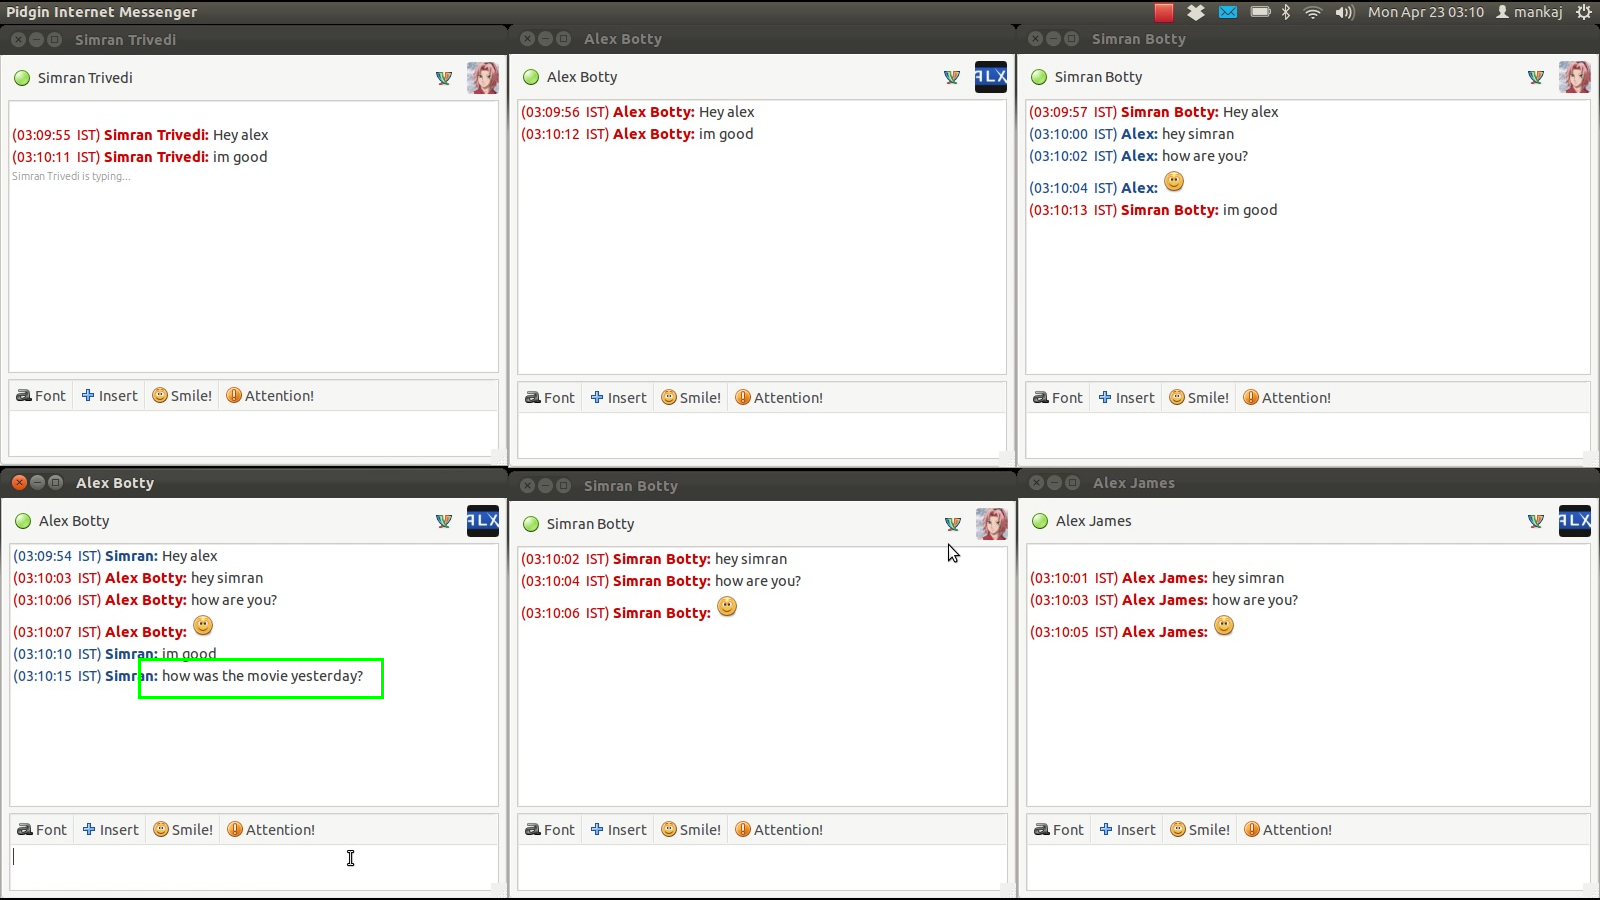
\includegraphics[scale=0.6, angle=90]{project/diagrams/attack3}
\caption{Facebook Chat Attack - 3}
\label{fig:attack1}
\end{figure}

\begin{figure}[H]
\centering
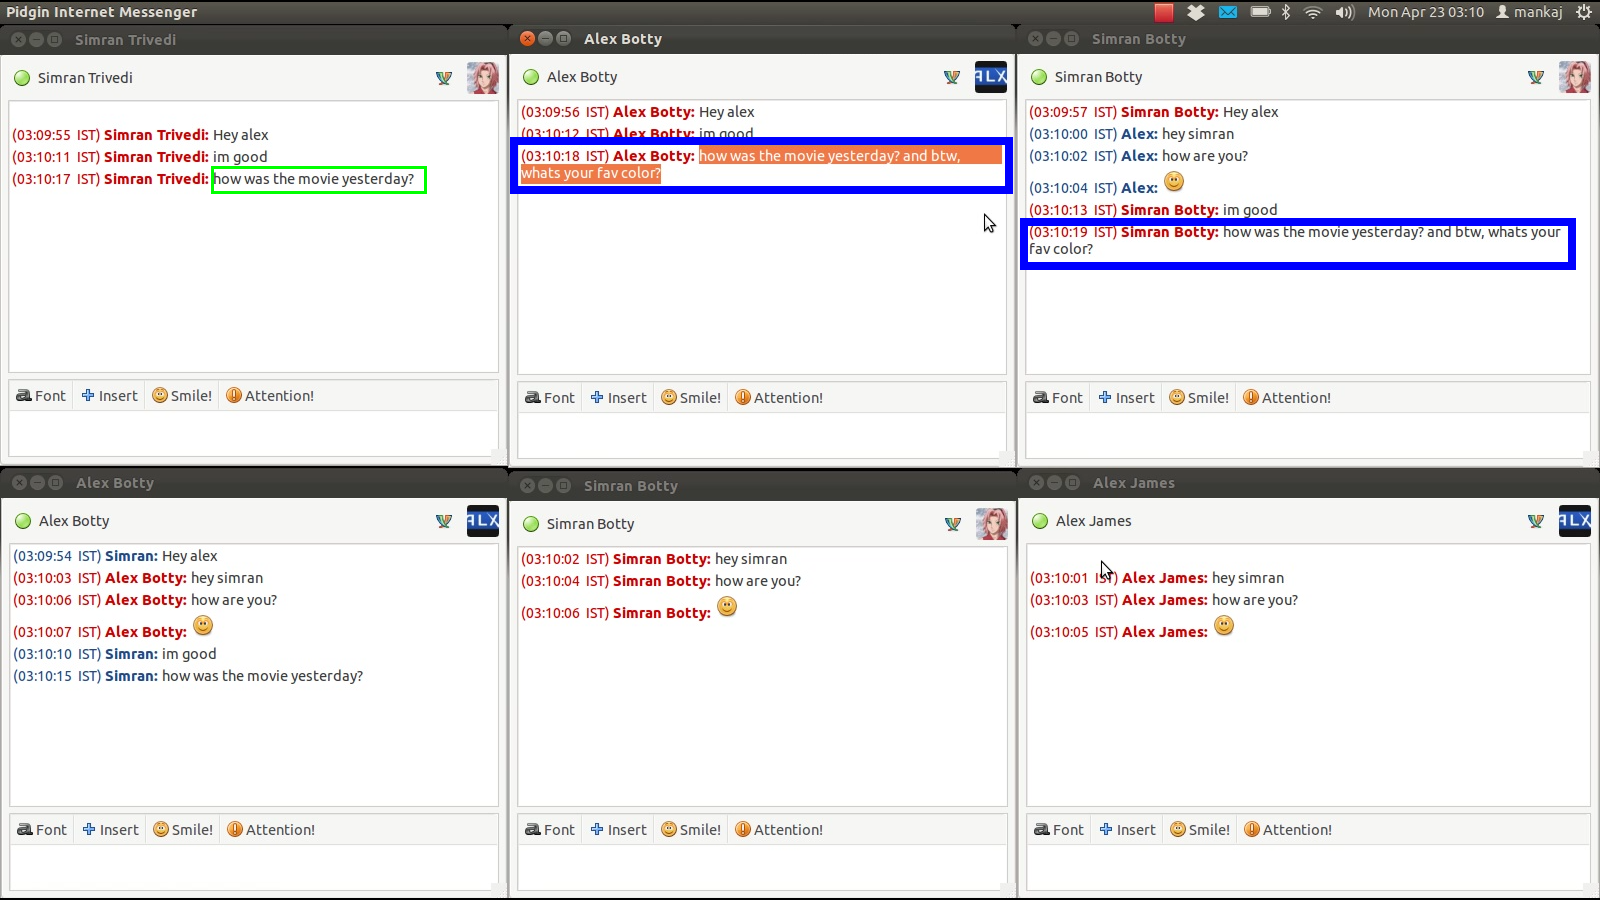
\includegraphics[scale=0.6, angle=90]{project/diagrams/attack4}
\caption{Facebook Chat Attack - 4}
\label{fig:attack1}
\end{figure}

\begin{figure}[H]
\centering
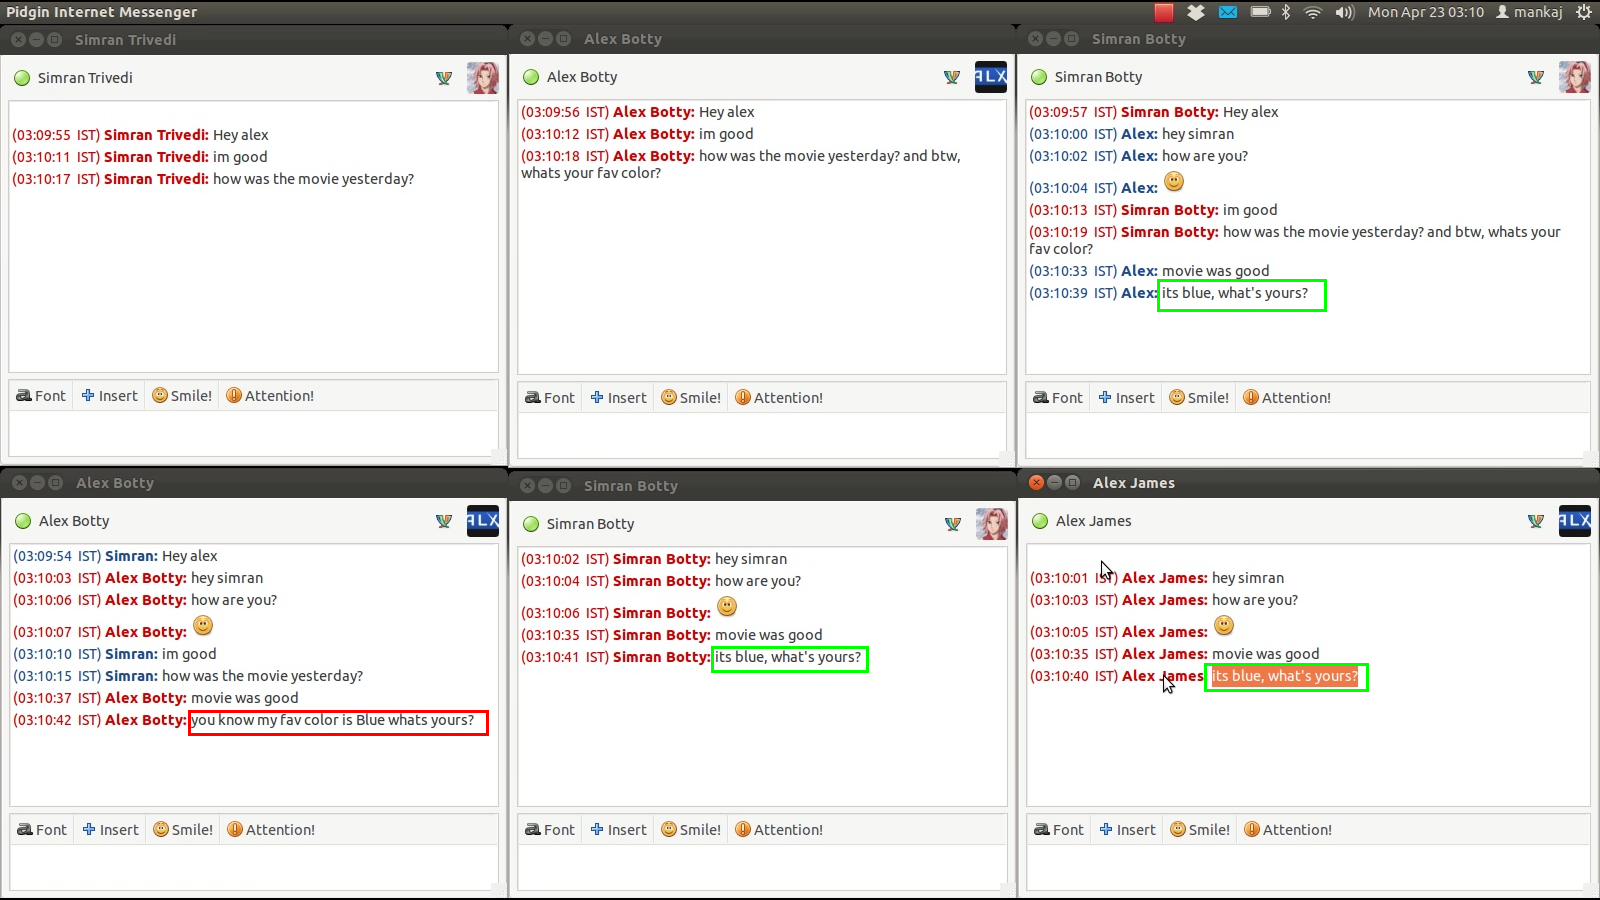
\includegraphics[scale=0.6, angle=90]{project/diagrams/attack5}
\caption{Facebook Chat Attack - 5}
\label{fig:attack1}
\end{figure}

\begin{figure}[H]
\centering
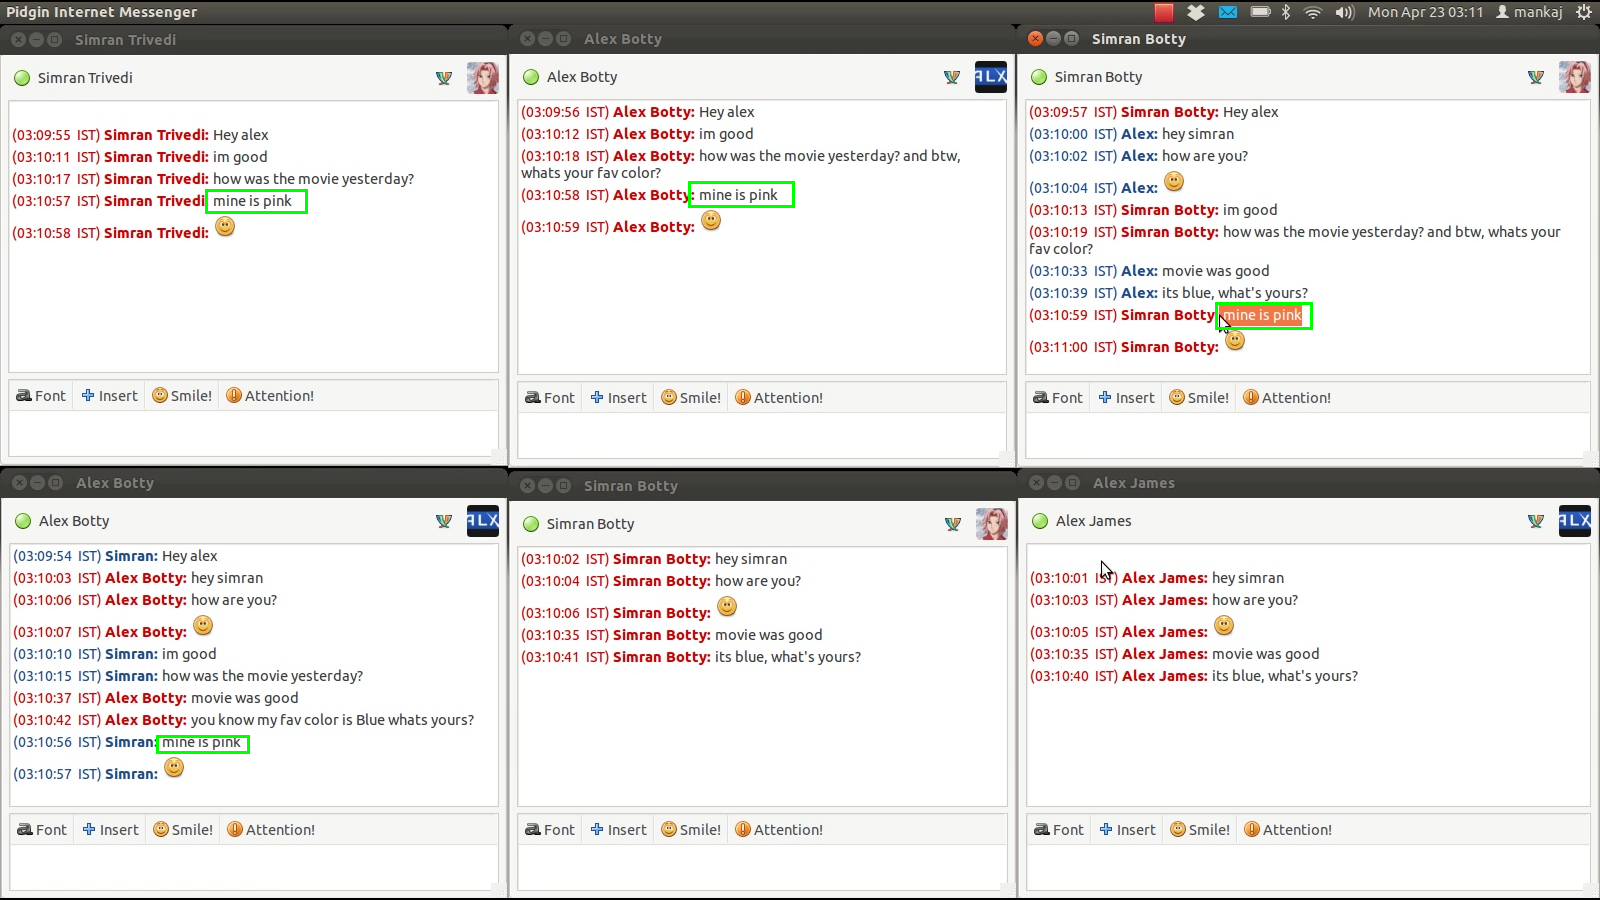
\includegraphics[scale=0.6, angle=90]{project/diagrams/attack6}
\caption{Facebook Chat Attack - 6}
\label{fig:attack1}
\end{figure}

 % adds the Project Design
\chapter{Scheduling}


\section{Proposed Modules}

\begin{itemize}
\item{Passive Information Gathering}
\item{Facebook Chat Attack}
\item{Modification of chat on the fly}
\end{itemize}

\section{Scheduling}

\begin{description}
\item[August-September 2011 : ] Finalized the Problem Statement
\item[September-October 2011 : ] Prepared SRS
\item[November-December 2011 : ] Exam Break
\item[December-January 2011-12 : ] Passive Information Gathering Module
\item[February 2012 : ] Learned XMPP, tried XMMPPPY Library and failed
\item[March 2012 : ] Learned SleekXMPP Python Library.
\item[March-April 2012 : ] Implemented Facebook Chat Attack
\item[April 2012 : ] Finished Project Report
\end{description}
 % adds the Scheduling and Planning page
\chapter{Conclusion and Future Scope}


\section{Future Scope}

The project certainly has a lot of scope. Let's take a look at some of them

\begin{itemize}
\item{We could extend the capabilities of extracting information to gather personal information as well like About Me page of the user.}
\item{Parallizes the HTTP request to make it faster}
\item{Deploy the passive information extractor on Amazon EC2 Servers.}
\item{Hook up AI bots like megahal\cite{wiki_megahal} in Facebook Chat Attack and train our scripts to learn when/what to modify}
\item{Feature to clone profiles}
\item{Scale the architecture where Facebook Chat Attack would work on more then just two people at the same time}
\end{itemize}

\section{Conclusion}
The project was sucessfully implemented and a Proof of Concept was established that Social Engineering can be done on Social Networks.\\
We were able to extract out public information from Facebook user's profile on a mass scale. Also we demonstrated that Trust between two users can be used to extract out information which is not available publicaly.

 % adds the Scheduling and Planning page
\addcontentsline{toc}{chapter}{References}
\begin{thebibliography}{99}

% \bibitem{TEXT} is how you refer to your reference in your report. keep that very short
% \emph{Paper Name} is just to highligh the paper name by making it italic, not required but looks nice

%Example
%\bibitem{short_paper_name}\emph{Paper Name}; Author Name, Conference Name, year etc 

\bibitem{paper_honeybot}\emph{Honeybot, Your Man in the Middle for Automated Social Engineering};Tobias Lauinger, Veikko Pankakoski, Davide Balzarotti, Engin Kirda; EURECOM Sophia-Antipolis, France. LEET’10 Proceedings of the 3rd USENIX conference on Large-scale exploits and emergent threats.

\bibitem{paper_allyourcontacts}\emph{All Your Contacts Are Belong to Us: Automated Identity Theft Attacks on Social Networks}; Leyla Bilge, Thorsten Strufe, Davide Balzarotti, Engin Kirda EURECOM Sophia Antipolis, France. WWW ’09 Proceedings of the 18th international conference on World Wide Web.

\bibitem{paper_eightfriends}\emph{Eight Friends Are Enough Social Graph Approximation via Public Listings}; Joseph Bonneau, Jonathan Anderson, Frank Stajano, Ross Anderson. SNS ’09: Proceedings of the Second ACM EuroSys Workshop on Social Network Systems.

\bibitem{paper_towardsautomating}\emph{Towards Automating Social Engineering Using Social Networking Sites};Huber, M.; Kowalski, S.; Nohlberg, M.; Tjoa, S.; Computational Science and Engineering, 2009. CSE ’09. International Conference.

\bibitem{book_se}Social Engineering : The art of Human Hacking


\bibitem{link_humanweak}Link Name \\ \url{http://goliath.ecnext.com/coms2/gi_0199-7186209/}
\url{The-human-element-the-weakest}


\bibitem{marketshare}Market Share of Social Network Sites \\ \url{http://techcrunch.com/2011/12/22/googlesplus}




%And how you would refer to the paper in the text - example
%Your text in other tex files \cite{short_paper_name} contd explaining

%If you have to display links, do it via  adding \\ (newline) otherwise it goes off the margins. Don't know how to fix this yet
%\bibitem{short_link_name}Link Name \\ \url{http://url link here}
%\url{The-human-element-the-weakest}



\end{thebibliography} % adds the References page

\end{document}
